%% Erläuterungen zu den Befehlen erfolgen unter
%% diesem Beispiel.

\documentclass{article}

\usepackage[utf8]{inputenc}
\usepackage[T1]{fontenc}
\usepackage{lmodern}
\usepackage[ngerman]{babel}
\usepackage{amsmath}
\usepackage{gensymb}
\usepackage{graphicx}

%% Helvetica als Schriftart benutzen
\usepackage{helvet} 
%%Schrift auf sans-serif setzen
\renewcommand{\familydefault}{\sfdefault}

\title{Dokumentation zum Arbeitsblatt 5 EWR}
\author{Tom Lambert}
\date{19. Juni 2017}
\begin{document}
	
	\maketitle
	\tableofcontents
	\newpage
	
	\section{Einführung in die Problemstellung}
	
	In der Vorlesung wurde in Abschnitt 11.3 folgende Aufgabe gestellt:
	
	\begin{quote}
		Bestimme die Koordinaten der Punkte auf der Einheitskreislinie.
	\end{quote}
	
	Dort wurden außerdem 3 Algorithmen vorgestellt, mit denen die Aufgabe gelöst werden kann. \\
	Diese und deren Implementierung werden später aufgezeigt.
	
	
	
	\section{Darstellung des theoretischen Hintergrunds}
	
	\subsection{Naiver Algorithmus}
	
	Wie einmal in der Schule kennen gelernt, kann man zum berechnen der Punkte auf dem Einheitskreis (in Abhängigkeit eines Winkels) mit Hilfe von Sinus und Cosinus verwenden.
	
	\begin{align}
		\begin{split}
			\label{eq:naiv}
			x(\alpha) &= \cos(2\pi\cdot \frac{\alpha}{360}) \\
			y(\alpha) &= \sin(2\pi\cdot \frac{\alpha}{360})
		\end{split}
	\end{align}
	
	Zur Berechnung von Sinus und Cosinus sind jedoch relativ aufwendige Rechnungen notwendig, die ggf. auch recht hohe Rundungsfehler aufweisen können. Die Berechnung aller Punkte auf diese Weiße ist daher "naiv".
	
	\subsection{Effizienter Algorithmus}
	
	Um die große Anzahl an Aufrufen von Sinus und Cosinus zu vermeiden, können die Gleichungen von (\ref{eq:naiv}) erweitert- und umgestellt werden.
	
	\begin{align}
	\beta &= \frac{2\pi}{360} & \tilde{\alpha} &= \frac{2\pi\alpha}{360} 
	\end{align}
	\begin{equation}
		\begin{split}		
			x(\alpha+1) &= \cos(2\pi \cdot \frac{\alpha}{360}+\frac{2\pi}{360}) =\cos{\tilde{\alpha}+\beta} \\
			   &= \cos(\tilde{\alpha})\cos(\beta) - \sin(\tilde{\alpha})\sin(\beta) \\
			y(\alpha+1) &= \sin(2\pi \cdot \frac{\alpha}{360}+\frac{2\pi}{360}) =\sin{\tilde{\alpha}+\beta} \\
			   &= \sin(\tilde{\alpha})\cos(\beta) - \cos(\tilde{\alpha})\sin(\beta) 
		\end{split}
	\end{equation}
	
	Dabei entspricht $\beta$ einem konstanten Wert, sodass dessen Sinus und Cosinus am Anfang nur je einmal berechnet werden müssen. Mehr als diese 2 Funktionsaufrufe entstehen nicht, da sich die weiteren Winkel aus dem vorher berechneten Punkt ergeben. 
	
	\subsection{Symmetrischer Algorithmus}
		
	
	Wenn mit Hilfe des naiven Algorithmus die Punkte zwischen 0 und 45 Grad berechnet werden, so ist leicht ersichtlich, dass die restlichen Punkte einfach durch spiegeln und drehen ermittelt werden können. Das Drehen meint hierbei eine einfache Vertauschung der x- und y-Werte, da lediglich um 90 Grad gedreht werden muss. Grafisch skizziert und in Gleichungen ausgedrückt meint dies:
	
	\begin{center}	
		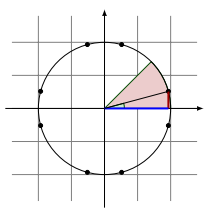
\includegraphics[width=3cm]{Images/sym.png}	
	\end{center}
	\begin{equation}
		\begin{split}
			\sin(\alpha) &= \sin(\pi-\alpha)  =-\sin(-\alpha) =-\sin(\pi+\alpha) \\
			\cos(\alpha) &= \cos(\pi-\alpha)  =-\cos(-\alpha)  =-\cos(\pi+\alpha)\\
			\sin(\alpha) &= \cos(\frac{\pi}{2}-\alpha) 
		\end{split}
	\end{equation}
	
	
	
	\section{Aufbau des Programs}
	
	Das Programm ist in mehrere Dateien untergliedert:
	
	\begin{enumerate}
		\item utils.py \\ Diese Datei enthält Hilfsfunktionen die in keinem näheren Zusammenhang mit dem eigentlichen Problem stehen. 
		\item kreis.py \\ Diese Datei enthält die Logik für die eigentlichen Berechnungen mit notwendigen, zusätzlichen Algorithmen für eine Auswertung.
		\item ab5.py \\ Diese Datei enthält das Hauptprogramm und enthält den Code, der die Tests durchführt.
	\end{enumerate}
	
	\subsection{utils.py}
	
	Diese Datei enthält Hilfsfunktionen die in keinem näheren Zusammenhang mit dem eigentlichen Problem stehen. Beispielsweise enthält sie eine Funktion \verb|average| zum Berechnen des Durchschnitts der Werte in einer Liste. Die Datei ist in früheren- bzw. späteren Entwicklungsstadien auch in anderen Projekten zu finden. Der Portabilität wegen wird sie stets kopiert anstatt sie aus einem anderen Ordner zu referenzieren.
	
	\subsection{kreis.py}
	
	Die Logik wurde mit Hilfe einer Klasse \verb|Kreis| realisiert, welche die notwendigen Methoden enthält.
	
	Zunächst bietet die Klasse 2 Funktionen \verb|_sin| und \verb|_cos|, welche einfach den Sinus bzw. Cosinus mit Hilfe der \verb|Sympy|-Bibliothek berechnen. Das besonder ist jedoch, dass ein Methodenaufruf auch einen internen Zähler um jeweils 1 erhöht. Über die \verb|function_call_counter|-Eigenschaft lässt sich dieser Zähler abfragen und ggf. über die \verb|reset_function_call_counter|-Funktion auf 0 zurück setzen. \\
	Dadurch wird es möglich von außen zu erfahren welcher Algorithmus wie oft Sinus- und Cosinus-Werte berechnet hat.
	
	Das eigentliche Kernstück sind jedoch die 3 Funktionen \verb|naiv|, \verb|effizient| sowie \verb|symmetrie|, die die Algorithmen implementieren. Allen gemeinsam ist, dass sie eine Liste mit Punkten auf dem Einheitskreis zurück geben. Und zwar genau 360 stück, einen Punkt je Grad. Weiterhin werden die Listen der Punkte als Wörterbuch zurück gegeben. Dadurch ist es möglich über einen als \verb|Key| gewählten Winkel einen bestimmten Punkt abzufragen.
	
	Zum Berechnen habe ich zunächst eine Hilfsfunktion \verb|_naiv(angles)| erstellt, welche eine Liste mit Punkten zurück gibt, die auf den übergebenen Winkeln liegen. Die \verb|naiv|-Funktion ruft \verb|_naiv| nun einfach mit einer Liste der 360 Winkel auf. 
	
	Die Funktion \verb|symmetrie| jedoch nur für die Winkel von 1 bis 45 Grad, sodass dann für jeden zurück gegebenen Punkt die 7 passend gespiegelt- und gedrehten Punkte ermittelt werden können.
	
	Die \verb|effizient|-Funktion arbeitet davon unabhängig. Sie ermittelt zunächst die konstanten Sinus- und Cosinus-Werte für den Winkel $\beta$ und initialisiert 2 Hilfsvariablen. In diesen werden die Koordinaten des zuletzt berechneten Punkts abgelegt. In einer Schleife werden nun Schritt für Schritt die einzelnen Punkte auf Basis des zuvor berechneten Punkts berechnet.
	
	
	\subsection{ab5.px}
	
	Diese Datei enthält als ausführbaren Code lediglich eine \verb|main|-Methode, welche direkt am Ende aufgerufen wird. Diese Implementierung hat den Vorteil, dass bei Erweiterung des Programms um Benutzereingaben einfach eine 2. Funktion implementiert werden kann.
	
	Innerhalb der \verb|main|-Funktion wird zunächst die Präzision des \verb|Decimal|-Typs auf 20 festgelegt. Anschließend wird ein Wörterbuch erstellt, welches einige vorberechnete Punkte des Einheitskreises enthält. Diese wurden mit Wolfram Mathematica auf 20 Nachkommastellen genau berechnet. Diese Werte dienen später zum Vergleich mit den dynamisch berechneten Werten und zum Ermitteln des absoluten und des relativen Fehlers.
	
	Zunächst werden nun die 3 Funktionen \verb|naiv|, \verb|effizient| und \verb|symmetrie| aufgerufen. Nach jedem Aufruf wird dabei \verb|function_call_counter| abgefragt, dem Benutzer ausgegeben und dann zurück gesetzt. So kann kontrolliert werden, wie oft Sinus und Cosinus-Werte berechnet wurden.
	Im zweiten Schritt werden nun einige ausgewählte berechnete Punkte mit ihren vorberechneten Pendants ausgegeben. Anschließend erscheinen die passenden absoluten- und relativen Fehler in der Benutzerausgabe. Während dieses Schritts werden die Fehler jeweils zu einer Liste hinzugefügt.
	
	Nach dem Durchlauf der Liste der ausgewählten Winkel werden noch die durchschnittlichen Fehler ausgegeben, um dem Benutzer ein besseres Gefühl zu verschaffen wie einzelne Werte in der Menge aller Fehler liegen.
	
	
	
	\section{Experimente, Beobachtungen und Auswertung}
	
	Die in \verb|ab5.py| implementierten Experimente wurden mit den Folgenden Winkeln (in Grad) durchgeführt: $\{0, 10, 22, 23, 45, 90, 280, 359\}$
	
	Der durchschnittliche absoluten Fehler lag beim naiven- und beim symmetrischen Algorithmus bei jeweils ca. $5\cdot10^{-17}$. Der effiziente Algorithmus erzielte einen durchschnittlichen absoluten Fehler von ca $2\cdot10^{-15}$ und war somit deutlich ungenauer als die anderen.
		
		Bei den relativen Fehlern ergab sich ein ähnliches Bild. Die geringsten Fehler entstanden beim symmetrischen Algorithmus mit eine Abweichung von um die $3\cdot 10^{-17}$. Der naive Algorithmus lag bei ca $4\cdot 10^{-16}$ und der effiziente bei $5\cdot 10^{-15}$.
	
	Wie zu erwarten war ruft der effiziente Algorithmus nur 2mal Sinus bzw. Cosinus auf und arbeitet somit potentiell am schnellsten. Der naive Algorithmus benötigt ganze 720 Aufrufe, wohingegen die Kompromiss-Lösung Symmetrie nur 92 Aufrufe braucht.
	
	Die Best-Practise Lösung ist für mich in den meisten Fällen die Symmetrie-Lösung. Sie ist in etwa genauso exakt wie die naive Lösung, in der Theorie jedoch deutlich performanter. Sollte eine Hohe Genauigkeit nicht erforderlich sein, so bietet sich jedoch auch weiterhin der Einsatz der effizienten Methode an.
	
	Aus der Sicht des Entwicklers ist der Wartungsaufwand beim naiven Algorithmus am geringsten, wobei auch der symmetrische keine großen Probleme machen sollte. Der effiziente Algorithmus benötigt jedoch ein wenig Einarbeitungszeit um ihn zu verstehen. Entsprechend würde eine Erweiterung hier schwieriger werden. Zu beachten sei weiterhin, dass der effiziente Algorithmus auf ganzen Winkeln (in Grad) aufbaut, die anderen beiden Konzepte jedoch auch mit gebrochenen Zahlen arbeiten können. Eine dahingehende Verallgemeinerung wäre nochmals deutlich aufwendiger.
	
\end{document}